% !TEX root = ../main.tex
% SECTION 9: MECHANISCHE MECHANISMEN
% Inhalt: Liv Erne, Silvio Seiz — Form: ZSF-Template-Rework
% ============================================================

\StartChapter[ch:mechanismen]{Mechanische Mechanismen}
\ZSFindex{Mechanismus}

\begin{runintext}
Kopplung von Elementen, bei der jede Bewegung eine andere bewirkt: Kraftverstärkung, Rotation zu Translation
\end{runintext}

\SubsectionBar[sec:force-amplification]{Kraftverstärkung}
\ZSFindex[kraftverstarkung]{Kraftverstärkung}

\begin{runintext}
$\rightarrow$ Weniger Kraft, mehr Weg: $W_1 = W_2$ also $F_1 \cdot s_1 = F_2 \cdot s_2$
\end{runintext}

\SubsubsectionBar{Hebel}
\ZSFindex{Hebel}

\begin{defbox}[Hebelgesetz \& Momentengleichgewicht]
  \ZSFkeyword{Momentengleichgewicht}:~Kräfte senkrecht auf Achse stellen.
  \ZSFgapXS
  {\centering
  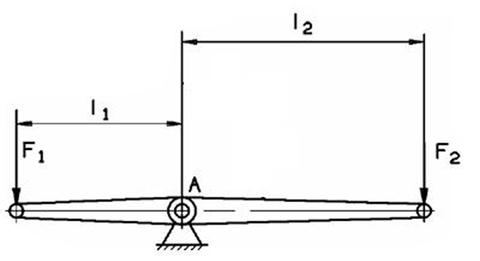
\includegraphics[width=0.48\linewidth,keepaspectratio]{graphics/v11_zweiseitiger_hebel.png}\hfill
  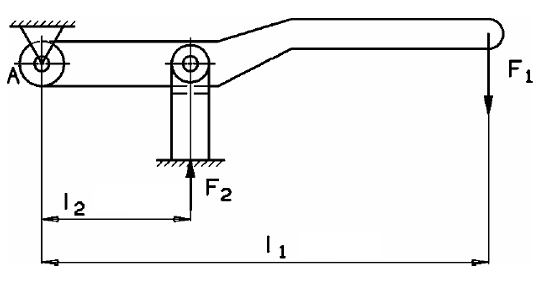
\includegraphics[width=0.48\linewidth,keepaspectratio]{graphics/v11_einseitiger_hebel.png}\par}
  \formulasep
  \ZSFkeyword*{Hebelgesetz}:~$\displaystyle F_2 = \frac{l_1}{l_2} \cdot F_1 = k \cdot F_1$
  \formulanote{Reihenschaltung: $\displaystyle F_3 = \frac{l_1}{l_2}\cdot \frac{l_3}{l_4} \cdot F_1 = k_1 \cdot k_2 \cdot F_1$}
\end{defbox}

\begin{defbox}[Kniehebel]
  \noindent
  \begin{minipage}[c]{0.16\linewidth}
    \centering
    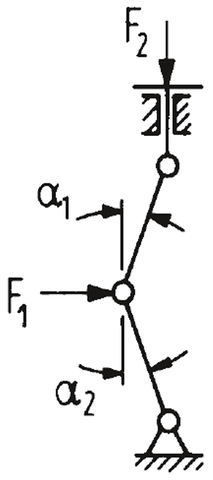
\includegraphics[width=\linewidth,keepaspectratio]{graphics/v11_toggle_lever_force_ratio.png}
  \end{minipage}%
  \hfill
  \begin{minipage}[c]{0.80\linewidth}
    \centering
    $\displaystyle
    \begin{aligned}
      F_2 &= \frac{F_1}{\tan\alpha_1 + \tan\alpha_2} = \frac{F_1}{2\cdot \tan\alpha} \\[4pt]
      K   &= \frac{1}{2\cdot \tan\alpha}
    \end{aligned}
    $
    \par\ZSFgapXS
    {\ZSFfontNote\ZSFmuted{$K$:~Kräfteverhältnis}}
  \end{minipage}
\end{defbox}
\ZSFindex{Kniehebel}

\begin{defbox}[Kniehebel-Spannvorrichtung (Beispiel)]
  \noindent
  \begin{minipage}[c]{0.38\linewidth}
    \centering
    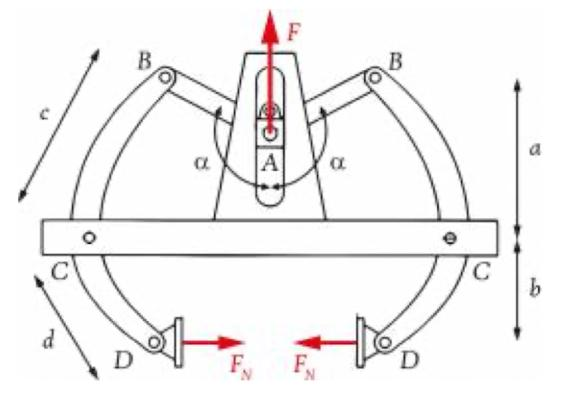
\includegraphics[width=\linewidth,keepaspectratio]{graphics/v11_kniehebel_spannvorrichtung_beispiel.jpeg}
  \end{minipage}%
  \hfill
  \begin{minipage}[c]{0.58\linewidth}
    \centering
    $\displaystyle
    \begin{aligned}
      F_N &= \frac{c \cdot F}{2\cdot \sin(\alpha - 90^\circ)\cdot b} \\[4pt]
          &= \frac{c \cdot F}{2\cdot \cos(180^\circ - \alpha)\cdot b}
    \end{aligned}
    $
  \end{minipage}
\end{defbox}

\SubsubsectionBar{Schiefe Ebene/ Keil}
\ZSFindex{Schiefe Ebene}
\ZSFindex{Keil}

\begin{figbox}
  \begin{minipage}[c]{0.44\linewidth}
    \centering
    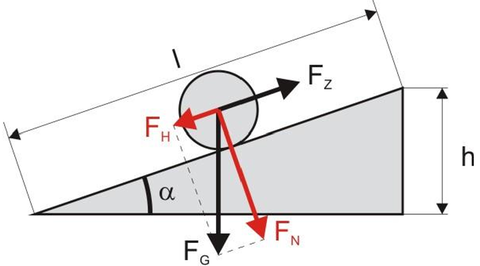
\includegraphics[width=\linewidth,keepaspectratio]{graphics/v11_inclined_plane_forces.png}
    $\displaystyle F_G = \frac{F_z}{\sin\alpha}$ \\[1pt]
    $\displaystyle F_2 = \frac{s_1}{s_2}{\cdot}F_1 = \frac{F_1}{\tan\alpha}$
  \end{minipage}\hfill
  \begin{minipage}[c]{0.52\linewidth}
    \centering
    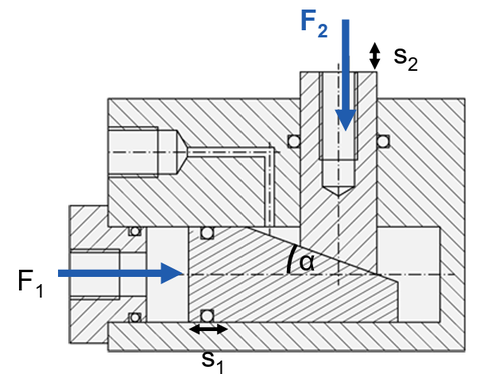
\includegraphics[width=\linewidth,keepaspectratio]{graphics/v11_wedge_force_ratio.png}
  \end{minipage}
\end{figbox}

\SubsubsectionBar{Schraube}

\begin{splitbox}[0.42]
\centering
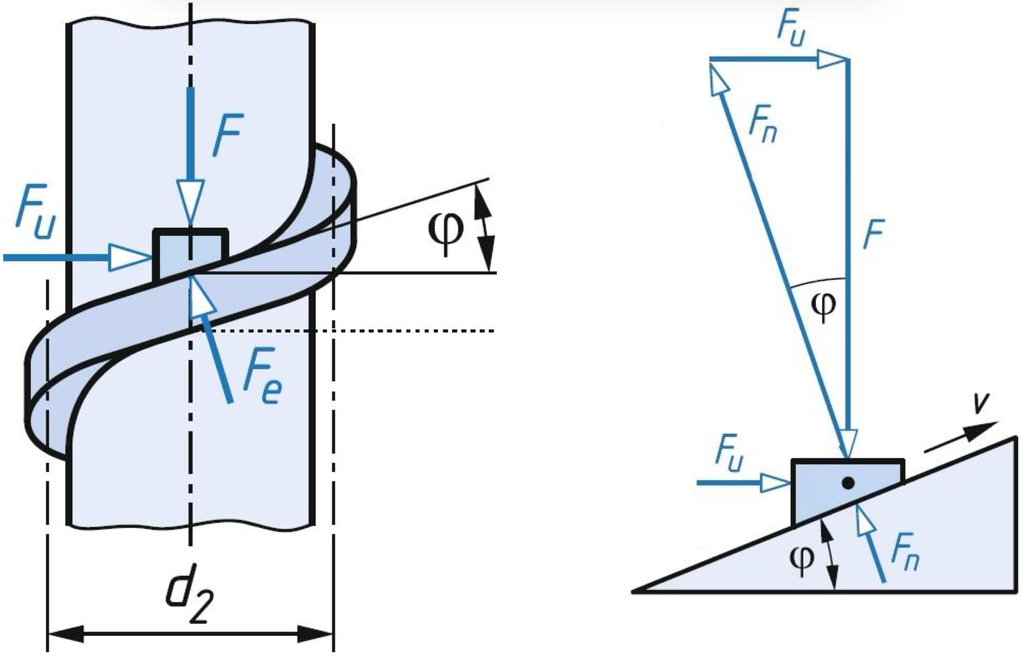
\includegraphics[width=\linewidth,keepaspectratio]{graphics/schraube_als_schiefe_ebene.png}
\tcblower
$\ZSFscrewF = \dfrac{\ZSFscrewFu}{\tan\ZSFscrewPhi}$

\ZSFmuted{Formel \ZSFsource{aus}{sec:schraubenbelastung}}
\end{splitbox}

\SubsubsectionBar{Flaschenzug}
\ZSFindex{Flaschenzug}

\begin{splitbox}[0.54]
\centering
\begin{tikzpicture}[x=1.35pt, y=1.35pt, >=latex, font=\sffamily\fontsize{4.5}{5.5}\selectfont]
  % Example 1: k=1 (Feste Rolle)
  \begin{scope}
    % Decke
    \draw[thick, gray] (1, 40) -- (13, 40);
    \foreach \x in {1,3,...,13} \draw[gray] (\x, 40) -- (\x+1.5, 42.5);

        % Aufhaengung feste Rolle (Ablenkrolle)
    \draw[very thick, ETHRot] (7, 40) -- (7, 30);
    \draw[ETHRot, thick] (5.5, 36.5) -- (8.5, 33.5);
    \draw[ETHRot, thick] (8.5, 36.5) -- (5.5, 33.5);

    % Rolle (weiss gefuellt)
    \draw[thick, fill=white] (7, 30) circle (4);
    \fill (7, 30) circle (1.2);

    % Seil (k=1)
    \draw[very thick, \chaptercolor] (3, 12) -- (3, 30);
    \draw[very thick, \chaptercolor] (3, 30) arc (180:0:4);
    \draw[very thick, \chaptercolor, ->] (11, 30) -- (16, 15) node[right, scale=0.8] {$\ZSFpulleyFZ$};

    % Last
    \draw[thick] (3, 12) -- (3, 7);
    \draw[thick, fill=black!10] (0, 7) rectangle (6, -1) node[pos=0.5, scale=0.8] {$\ZSFpulleyFL$};

    % Annotations
    \node[circle, fill=\chaptercolorlight!80, text=\chaptercolor, font=\tiny\bfseries, inner sep=1pt] at (1, 21) {1};
    \node[circle, fill=\chaptercolorlight!80, text=\chaptercolor, font=\tiny\bfseries, inner sep=1pt] at (15, 20) {1};
    \node[circle, fill=MathHLTertiary!15, text=MathHLTertiary, font=\tiny\bfseries, inner sep=1.2pt] at (3, 9.5) {1};
    \node[below, scale=0.8] at (3, -1) {\textbf{$\ZSFpulleyK = 1$}};
  \end{scope}

  % Example 2: k=2 (Faktorenflaschenzug)
  \begin{scope}
    % Decke
    \draw[thick, gray] (21, 40) -- (33, 40);
    \foreach \x in {21,23,...,33} \draw[gray] (\x, 40) -- (\x+1.5, 42.5);

    % Aufhaengung feste Rolle (Ablenkrolle)
    \draw[very thick, ETHRot] (27, 40) -- (27, 30);
    \draw[ETHRot, thick] (25.5, 36.5) -- (28.5, 33.5);
    \draw[ETHRot, thick] (28.5, 36.5) -- (25.5, 33.5);

    % Rollen
    \draw[thick, fill=white] (27, 30) circle (4);
    \fill (27, 30) circle (1.2);
    \draw[thick, fill=white] (27, 15) circle (4);
    \fill (27, 15) circle (1.2);

    % Seil 1 (k=2)
    \draw[very thick, \chaptercolor] (27, 30) -- (23, 15);
    \draw[very thick, \chaptercolor] (23, 15) arc (180:360:4);
    \draw[very thick, \chaptercolor] (31, 15) -- (31, 30);
    \draw[very thick, \chaptercolor] (31, 30) arc (0:180:4);
    \draw[very thick, \chaptercolor, ->] (23, 30) -- (18, 15) node[left, scale=0.8] {$\ZSFpulleyFZ$};

    % Last
    \draw[thick] (27, 15) -- (27, 7);
    \draw[thick, fill=black!10] (24, 7) rectangle (30, -1) node[pos=0.5, scale=0.8] {$\ZSFpulleyFL$};

    % Annotations
    \node[circle, fill=\chaptercolorlight!80, text=\chaptercolor, font=\tiny\bfseries, inner sep=1pt] at (20, 20) {1};
    \node[circle, fill=\chaptercolorlight!80, text=\chaptercolor, font=\tiny\bfseries, inner sep=1pt] at (24.6, 22) {1};
    \node[circle, fill=\chaptercolorlight!80, text=\chaptercolor, font=\tiny\bfseries, inner sep=1pt] at (33, 22) {1};
    \node[circle, fill=MathHLTertiary!15, text=MathHLTertiary, font=\tiny\bfseries, inner sep=1.2pt] at (27, 11) {2};
    \node[below, scale=0.8] at (27, -1) {\textbf{$\ZSFpulleyK = 2$}};
  \end{scope}

  % Example 3: k=4 (Potenzierter Flaschenzug)
  \begin{scope}
    % Decke
    \draw[thick, gray] (39, 48) -- (65, 48);
    \foreach \x in {39,41,...,65} \draw[gray] (\x, 48) -- (\x+1.5, 50.5);

    % Aufhaengung feste Rolle (Ablenkrolle)
    \draw[very thick, ETHRot] (45, 48) -- (45, 35);
    \draw[ETHRot, thick] (43.5, 43) -- (46.5, 40);
    \draw[ETHRot, thick] (46.5, 43) -- (43.5, 40);

    % Rollen
    \draw[thick, fill=white] (45, 35) circle (4);
    \fill (45, 35) circle (1.2);

    \draw[thick, fill=white] (53, 25) circle (4);
    \fill (53, 25) circle (1.2);

    \draw[thick, fill=white] (57, 10) circle (4);
    \fill (57, 10) circle (1.2);

    % Seil 1 (Teal)
    \draw[very thick, \chaptercolor] (57, 48) -- (57, 25);
    \draw[very thick, \chaptercolor] (57, 25) arc (0:-180:4);
    \draw[very thick, \chaptercolor] (49, 25) -- (49, 35);
    \draw[very thick, \chaptercolor] (49, 35) arc (0:180:4);
    \draw[very thick, \chaptercolor, ->] (41, 35) -- (36, 15) node[left, scale=0.8] {$\ZSFpulleyFZ$};

    % Seil 2 (Orange)
    \draw[very thick, MathHLSecondary] (53, 25) -- (53, 10);
    \draw[very thick, MathHLSecondary] (53, 10) arc (180:360:4);
    \draw[very thick, MathHLSecondary] (61, 10) -- (61, 48);

    % Last
    \draw[thick] (57, 10) -- (57, 2);
    \draw[thick, fill=black!10] (53, 2) rectangle (61, -6) node[pos=0.5, scale=0.8] {$\ZSFpulleyFL$};

    % Annotations
    \node[circle, fill=\chaptercolorlight!80, text=\chaptercolor, font=\tiny\bfseries, inner sep=1pt] at (38, 20) {1};
    \node[circle, fill=\chaptercolorlight!80, text=\chaptercolor, font=\tiny\bfseries, inner sep=1pt] at (47.5, 30) {1};
    \node[circle, fill=\chaptercolorlight!80, text=\chaptercolor, font=\tiny\bfseries, inner sep=1pt] at (58.5, 33) {1};
    \node[circle, fill=MathHLSecondary!15, text=MathHLSecondary, font=\tiny\bfseries, inner sep=1pt] at (51.5, 18) {2};
    \node[circle, fill=MathHLSecondary!15, text=MathHLSecondary, font=\tiny\bfseries, inner sep=1pt] at (62.5, 25) {2};
    \node[circle, fill=MathHLTertiary!15, text=MathHLTertiary, font=\tiny\bfseries, inner sep=1.2pt] at (57, 5) {4};
    \node[below, scale=0.8] at (57, -6) {\textbf{$\ZSFpulleyK = 4$}};
  \end{scope}

  % Warning Box: Ablenkrolle (unter Example 1 & 2)
  \begin{scope}[shift={(0,-52)}]
    % Decke
    \draw[thick, gray] (11, 40) -- (23, 40);
    \foreach \x in {11,13,...,23} \draw[gray] (\x, 40) -- (\x+1.5, 42.5);

    % Feste Rolle Support (Ablenkrolle)
    \draw[very thick, ETHRot] (17, 40) -- (17, 30);
    \node[right, ETHRot, scale=0.7, font=\bfseries] at (18, 35) {Ablenkrolle};

    % Pulley
    \draw[thick, fill=white] (17, 30) circle (4);
    \fill (17, 30) circle (1.2);

    % Rope
    \draw[very thick, \chaptercolor] (13, 20) -- (13, 30);
    \draw[very thick, \chaptercolor] (13, 30) arc (180:0:4);
    \draw[very thick, \chaptercolor, ->] (21, 30) -- (26, 15) node[right, scale=0.8] {$\ZSFpulleyFZ$};

    % Red cross on the support
    \draw[ETHRot, thick] (15.5, 36.5) -- (18.5, 33.5);
    \draw[ETHRot, thick] (18.5, 36.5) -- (15.5, 33.5);

    % Annotations
    \node[circle, fill=\chaptercolorlight!80, text=\chaptercolor, font=\tiny\bfseries, inner sep=1pt] at (11, 25) {1};
    \node[circle, fill=\chaptercolorlight!80, text=\chaptercolor, font=\tiny\bfseries, inner sep=1pt] at (25, 23) {1};
  \end{scope}
\end{tikzpicture}
\tcblower
\ZSFReadableOn
\ZSFkeyword{Kraftzahl-Methode} zur Bestimmung von \mbox{$\ZSFpulleyFZ = \ZSFpulleyFL / \ZSFpulleyK$}:
\begin{enumerate}[leftmargin=1.1em, itemsep=1.5pt, parsep=0pt, topsep=1pt]
  \item \textbf{\color{\chaptercolor}Zugende = 1}: Das Seilende am Kraftangriff $\ZSFpulleyFZ$ erh\"alt die Kraftzahl \textcolor{\chaptercolor}{\textbf{1}}.
  \item \textbf{\color{\chaptercolor}Gleiches Seil}: Ein ununterbrochenes Seil hat \"uberall dieselbe Kraftzahl.
  \item \textbf{\color{MathHLSecondary}Rollen-Summe}: Eine lose Rolle addiert die Werte ihrer tragenden Seile auf ihre Aufh\"angung (z.\,B. \mbox{\textcolor{MathHLSecondary}{\textbf{2}} = \textcolor{\chaptercolor}{\textbf{1}} + \textcolor{\chaptercolor}{\textbf{1}}}).
  \item \textbf{\color{MathHLTertiary}Last-Summe $\ZSFpulleyK$}: Die Summe aller an der Last ziehenden Seilwerte ergibt \textbf{$\ZSFpulleyK$}.
\end{enumerate}
\par\ZSFgapXS
\ZSFdanger{Ablenkrollen} (fest an Decke) \"andern nur die Richtung und tragen nicht zu \textbf{$\ZSFpulleyK$} bei!
\end{splitbox}


\SubsectionBar[sec:rotation-translation]{Rotation zu Translation}

\SubsubsectionBar{Schubkurbel (Slider Crank)}
\ZSFindex{Schubkurbel}
\ZSFindexsee{Slider Crank}{Schubkurbel}

\begin{runintext}
Tangentialkraft $\ZSFmechFt$ der Kurbel (Rotation) führt zu Kraft im Pleuel $\ZSFmechFp$, führt zu Kraft im Stössel $\ZSFmechFs$ (Translation).
\end{runintext}

\begin{defbox}[Zentrische Schubkurbel]
  {\centering
  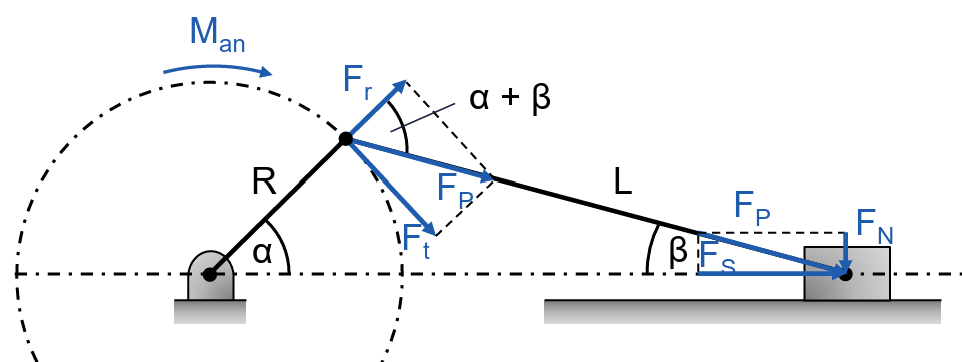
\includegraphics[width=0.85\linewidth,keepaspectratio]{graphics/v11_zentrische_schubkurbel.png}\par}
  \formulasep
  \centering
  $\displaystyle
  \begin{aligned}
    \ZSFmechH &= 2\cdot \ZSFmechR & \ZSFmechT &= \frac{1}{\ZSFmechN} = \frac{60s}{40} \quad (\text{wenn } \ZSFmechN = 40\text{min}^{-1}) \\[4pt]
    \ZSFmechGamma &= \frac{\ZSFmechR}{\ZSFmechL} = \frac{\sin\ZSFmechBeta}{\sin\ZSFmechAlpha} & \ZSFmechFs &= \frac{\cos\ZSFmechBeta \cdot \ZSFmechMan}{\sin(\ZSFmechAlpha+\ZSFmechBeta)\cdot \ZSFmechR}
  \end{aligned}
  $
  \par\ZSFgapXS
  \formulanote{$\ZSFmechH$:~Hub, $\ZSFmechT$:~Taktzeit ($360^\circ$), $\ZSFmechGamma$:~Schubstangenverhältnis ($\frac{R}{L}$, kleiner $\implies$ gleichförmiger), $\ZSFmechR$:~Kurbelradius, $\ZSFmechL$:~Pleuellänge, $\ZSFmechAlpha$/$\ZSFmechBeta$:~Kurbel-/Pleuelwinkel, $\ZSFmechFs$:~Stösselkraft, $\ZSFmechMan$:~Antriebsmoment, $\ZSFmechN$:~Drehzahl}
\end{defbox}

\begin{defbox}[Exzentrische Schubkurbel (Quick-Return)]
  {\centering
  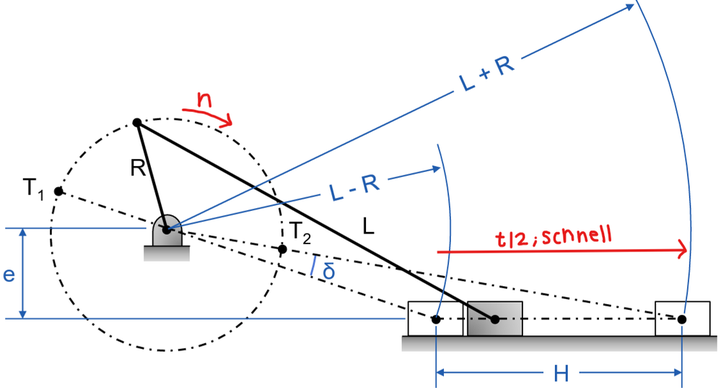
\includegraphics[width=0.70\linewidth,keepaspectratio]{graphics/v11_exzentrische_schubkurbel_quick_return.png}\par}
  \formulasep
  \ZSFkeyword{Zeitenverhältnis} $\ZSFmechQ$:~\par\ZSFgapXS
  \centering
  $\displaystyle \ZSFmechQ = \frac{\ZSFmechTslow}{\ZSFmechTfast} = \frac{180^\circ + \ZSFmechDelta}{180^\circ - \ZSFmechDelta}
  \quad \ZSFmechDelta = 180^\circ \cdot \frac{\ZSFmechQ - 1}{\ZSFmechQ+1}
  \quad \ZSFmechTges = \ZSFmechTslow + \ZSFmechTfast = \frac{1}{\ZSFmechN}$ \\[4pt]
  $\displaystyle \ZSFmechTfast = \frac{180^\circ - \ZSFmechDelta}{360^\circ} \cdot \frac{60}{\ZSFmechN}
  \quad \ZSFmechTslow = \frac{180^\circ + \ZSFmechDelta}{360^\circ} \cdot \frac{60}{\ZSFmechN}$
  \par\ZSFgapS
  \begin{factlist}
    \item Falls Winkel zwischen $T_1$ und $T_2 < 180^\circ \rightarrow$ schnell
    \item Falls Winkel zwischen $T_1$ und $T_2 > 180^\circ \rightarrow$ langsam
    \item $\ZSFmechEcc \uparrow \implies \ZSFmechDelta \uparrow \implies \ZSFmechQ \uparrow$
  \end{factlist}
  \par\ZSFgapXS
  \formulanote{$\ZSFmechQ$:~Zeitenverhältnis, $\ZSFmechTslow$/$\ZSFmechTfast$:~Zeit langsam/schnell, $\ZSFmechDelta$:~Symmetriewinkel, $\ZSFmechEcc$:~Exzentrizität}
\end{defbox}
\ZSFindex{Quick-Return}

\SubsubsectionBar{Kurbelschleife (Quick-Return)}
\ZSFindex{Kurbelschleife}

\begin{splitbox}[0.55]
\centering
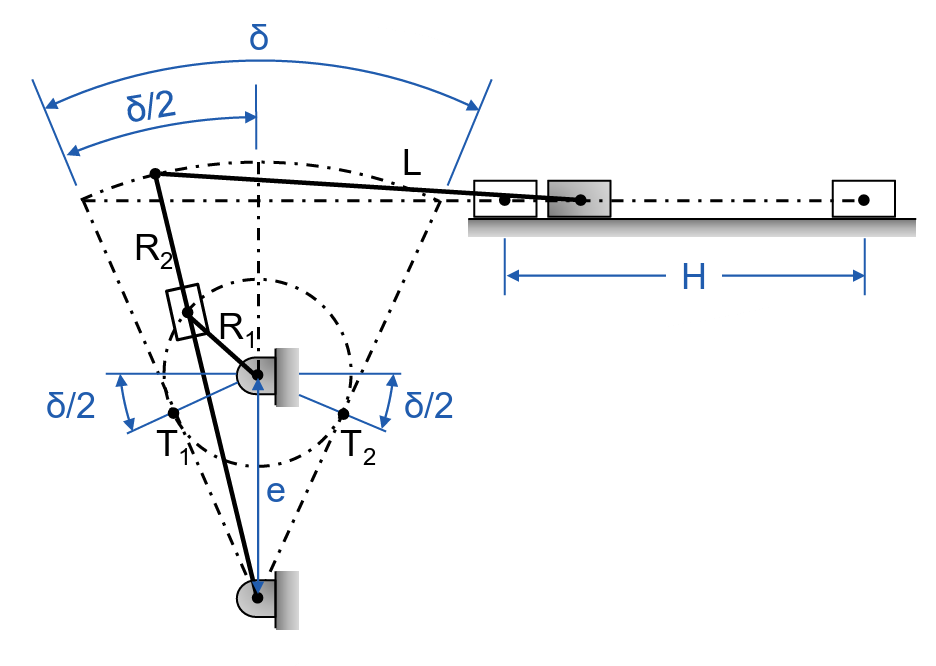
\includegraphics[width=\linewidth,keepaspectratio]{graphics/v11_kurbelschleife_quick_return.png}
\tcblower
$\sin(\dfrac{\ZSFmechDelta}{2})= \dfrac{\ZSFmechROne}{\ZSFmechEcc} = \dfrac{\ZSFmechH}{2\cdot \ZSFmechRTwo}$

$\ZSFmechQ = \dfrac{180° + \ZSFmechDelta}{180° - \ZSFmechDelta}$

$\ZSFmechTslow/\ZSFmechTfast = \dfrac{180° \pm \ZSFmechDelta}{360°} \cdot \dfrac{60}{\ZSFmechN}$
\par\ZSFgapXS
\formulanote{$\ZSFmechROne$:~Antriebsradius, $\ZSFmechRTwo$:~Schwingenlänge, $\ZSFmechEcc$:~Pivot-Abstand}
\end{splitbox}


\SubsubsectionBar{Viergelenkkette (Four Bar Linkage)}
\ZSFindex{Viergelenkkette}
\ZSFindexsee{Four Bar Linkage}{Viergelenkkette}

\begin{splitbox}[0.38]
\ZSFindex[drehfahigkeit]{Drehfähigkeit}
\ZSFkeyword*{Drehfähigkeit}:~"Die Kurbel ist voll drehfähig, wenn die Summe des kleinsten und grössten Stabes kleiner als die Summe der mittleren Stäbe ist."
\par\ZSFgapXS
{\ZSFfontNote \textbf{Grenzgetriebe} (durchschlagend): Summe zweier Stäbe = Summe der anderen}
\par\ZSFgapXS
{\sffamily\fontsize{5.8bp}{6.3bp}\selectfont
\begin{enumerate}[leftmargin=1.0em, itemsep=0.5pt, parsep=0pt, topsep=1pt]
  \item Kurbelschwinge
  \item Kurbelschwinge
  \item durchsch. Kurbelschwinge
  \item durchsch. Kurbelschwinge
  \item Kurbelschwinge
  \item Parallelkurbelgetriebe
  \item durchsch. Kurbelschwinge
\end{enumerate}
}
\tcblower
\centering
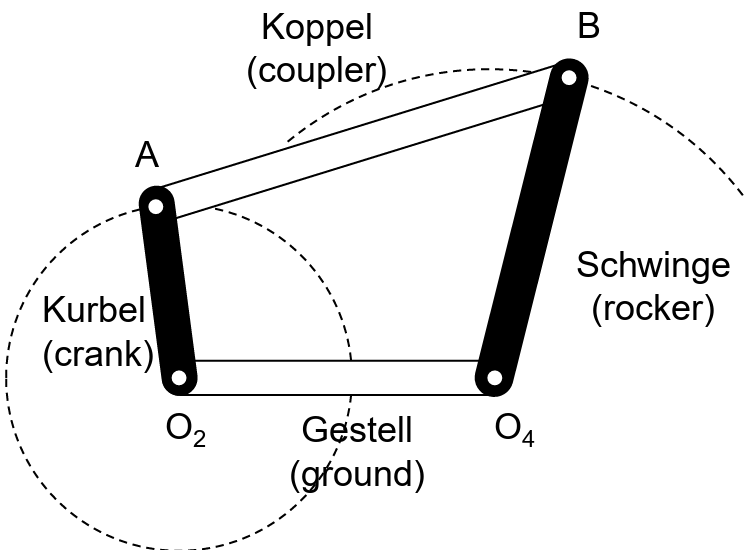
\includegraphics[width=0.86\linewidth,keepaspectratio]{graphics/v11_viergelenkkette_four_bar_linkage.png}
\end{splitbox}






\ZSFfig[1.0]{graphics/v11_four_bar_rotatability_cases.png}{}{}

\SubsubsectionBar{Koppelgetriebe}
\ZSFindex{Koppelgetriebe}

% Spalten-Packung (6-Seiten-Ziel): Bilderstapel in zwei figboxen geteilt,
% damit die Teile an Spaltenenden umbruchfähig sind. Bildgrössen unverändert.
\begin{figbox}
\centering
% kein \quad: 0.35+0.62+quad > Zeilenbreite -> Bilder wuerden untereinander rutschen
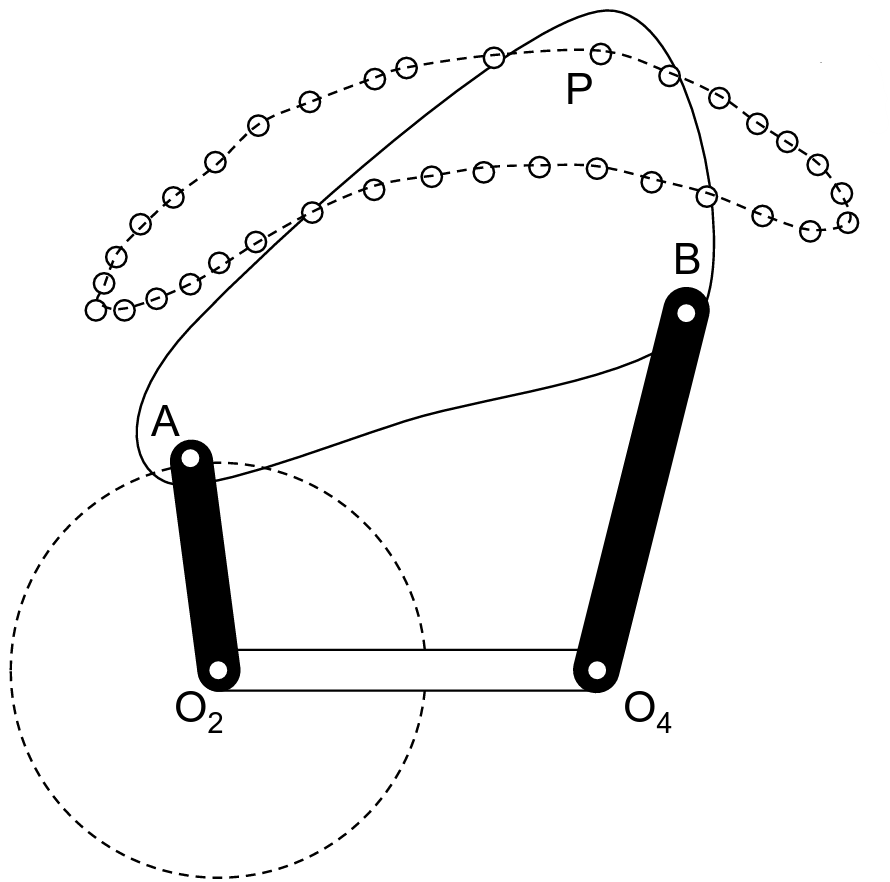
\includegraphics[width=0.35\linewidth,keepaspectratio]{graphics/v11_koppelkurve.png}
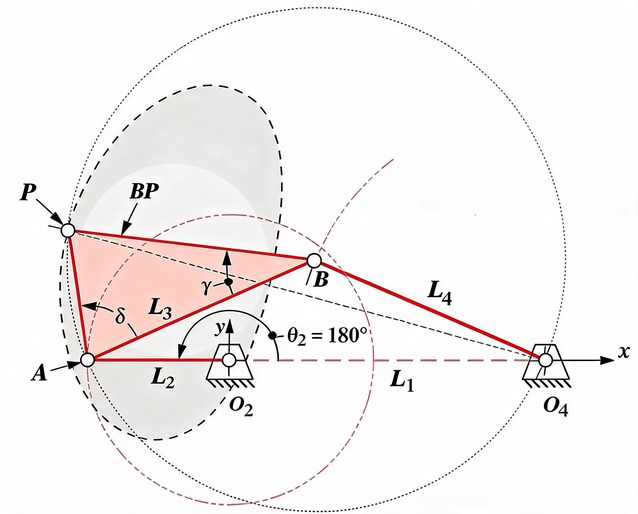
\includegraphics[width=0.62\linewidth,keepaspectratio]{graphics/v11_coupler_mechanism_lengths_angles.jpg}
\end{figbox}
